% Drawing 74/05-11 -- folder 74, batch 05, archive page 87 (PDF page 88).
% Transcription: Les quatre sommets $(ba')$, $(bb')$, $(aa')$, $(ab')$ disposés en carré, reliés par les deux diagonales qui se croisent.
% Kind: four vertices in a square with crossing diagonals. Method 2 (schematic redraw from the facsimile). Status: ok.
% Notes: (ba'), (bb') on top, (aa'), (ab') below; the two diagonals crossing (overinked); the sides are drawn as short strokes between the labels, as on the page.
% Coordinates: 1 unit = 1 mm = 1/100 of the crop width (bbox in page fractions: [0.35, 0.21, 0.62, 0.32]).
% Redrawn by Claude (claude-opus-5-5), issue #73, 2026-11-07; not checked by a human; not compiled (no TeX in the session).
% Rights: reproduces part of the work -- behind RENDER_TRANSCRIPTS, never published by itself.
\documentclass[tikz,border=3pt]{standalone}
\usepackage{amsmath,amssymb}
\usetikzlibrary{patterns,arrows.meta}
\tikzset{pencil/.style={black!45}, struck/.style={black!35}, mark/.style={circle,draw,inner sep=1.3pt}, pt/.style={circle,fill,inner sep=0.9pt}, opt/.style={circle,draw,fill=white,inner sep=1.1pt}}
\begin{document}
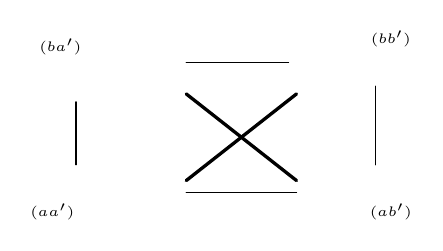
\begin{tikzpicture}[x=1mm,y=1mm,line cap=round,line join=round,font=\scriptsize]
\node[inner sep=1pt] at (36,-25) {\tiny $(ba')$};
\node[inner sep=1pt] at (78,-24) {\tiny $(bb')$};
\node[inner sep=1pt] at (35,-46) {\tiny $(aa')$};
\node[inner sep=1pt] at (78,-46) {\tiny $(ab')$};
\draw (52,-27) -- (65,-27);
\draw (52,-43.5) -- (66,-43.5);
\draw (38,-32) -- (38,-40);
\draw (76,-30) -- (76,-40);
\draw[very thick] (52,-31) -- (66,-42);
\draw[very thick] (52,-42) -- (66,-31);
\end{tikzpicture}
\end{document}
